% Options for packages loaded elsewhere
% Options for packages loaded elsewhere
\PassOptionsToPackage{unicode}{hyperref}
\PassOptionsToPackage{hyphens}{url}
\PassOptionsToPackage{dvipsnames,svgnames,x11names}{xcolor}
%
\documentclass[
  letterpaper,
  DIV=11,
  numbers=noendperiod]{scrreprt}
\usepackage{xcolor}
\usepackage{amsmath,amssymb}
\setcounter{secnumdepth}{5}
\usepackage{iftex}
\ifPDFTeX
  \usepackage[T1]{fontenc}
  \usepackage[utf8]{inputenc}
  \usepackage{textcomp} % provide euro and other symbols
\else % if luatex or xetex
  \usepackage{unicode-math} % this also loads fontspec
  \defaultfontfeatures{Scale=MatchLowercase}
  \defaultfontfeatures[\rmfamily]{Ligatures=TeX,Scale=1}
\fi
\usepackage{lmodern}
\ifPDFTeX\else
  % xetex/luatex font selection
\fi
% Use upquote if available, for straight quotes in verbatim environments
\IfFileExists{upquote.sty}{\usepackage{upquote}}{}
\IfFileExists{microtype.sty}{% use microtype if available
  \usepackage[]{microtype}
  \UseMicrotypeSet[protrusion]{basicmath} % disable protrusion for tt fonts
}{}
\makeatletter
\@ifundefined{KOMAClassName}{% if non-KOMA class
  \IfFileExists{parskip.sty}{%
    \usepackage{parskip}
  }{% else
    \setlength{\parindent}{0pt}
    \setlength{\parskip}{6pt plus 2pt minus 1pt}}
}{% if KOMA class
  \KOMAoptions{parskip=half}}
\makeatother
% Make \paragraph and \subparagraph free-standing
\makeatletter
\ifx\paragraph\undefined\else
  \let\oldparagraph\paragraph
  \renewcommand{\paragraph}{
    \@ifstar
      \xxxParagraphStar
      \xxxParagraphNoStar
  }
  \newcommand{\xxxParagraphStar}[1]{\oldparagraph*{#1}\mbox{}}
  \newcommand{\xxxParagraphNoStar}[1]{\oldparagraph{#1}\mbox{}}
\fi
\ifx\subparagraph\undefined\else
  \let\oldsubparagraph\subparagraph
  \renewcommand{\subparagraph}{
    \@ifstar
      \xxxSubParagraphStar
      \xxxSubParagraphNoStar
  }
  \newcommand{\xxxSubParagraphStar}[1]{\oldsubparagraph*{#1}\mbox{}}
  \newcommand{\xxxSubParagraphNoStar}[1]{\oldsubparagraph{#1}\mbox{}}
\fi
\makeatother


\usepackage{longtable,booktabs,array}
\usepackage{calc} % for calculating minipage widths
% Correct order of tables after \paragraph or \subparagraph
\usepackage{etoolbox}
\makeatletter
\patchcmd\longtable{\par}{\if@noskipsec\mbox{}\fi\par}{}{}
\makeatother
% Allow footnotes in longtable head/foot
\IfFileExists{footnotehyper.sty}{\usepackage{footnotehyper}}{\usepackage{footnote}}
\makesavenoteenv{longtable}
\usepackage{graphicx}
\makeatletter
\newsavebox\pandoc@box
\newcommand*\pandocbounded[1]{% scales image to fit in text height/width
  \sbox\pandoc@box{#1}%
  \Gscale@div\@tempa{\textheight}{\dimexpr\ht\pandoc@box+\dp\pandoc@box\relax}%
  \Gscale@div\@tempb{\linewidth}{\wd\pandoc@box}%
  \ifdim\@tempb\p@<\@tempa\p@\let\@tempa\@tempb\fi% select the smaller of both
  \ifdim\@tempa\p@<\p@\scalebox{\@tempa}{\usebox\pandoc@box}%
  \else\usebox{\pandoc@box}%
  \fi%
}
% Set default figure placement to htbp
\def\fps@figure{htbp}
\makeatother





\setlength{\emergencystretch}{3em} % prevent overfull lines

\providecommand{\tightlist}{%
  \setlength{\itemsep}{0pt}\setlength{\parskip}{0pt}}



 


\KOMAoption{captions}{tableheading}
\makeatletter
\@ifpackageloaded{bookmark}{}{\usepackage{bookmark}}
\makeatother
\makeatletter
\@ifpackageloaded{caption}{}{\usepackage{caption}}
\AtBeginDocument{%
\ifdefined\contentsname
  \renewcommand*\contentsname{Table of contents}
\else
  \newcommand\contentsname{Table of contents}
\fi
\ifdefined\listfigurename
  \renewcommand*\listfigurename{List of Figures}
\else
  \newcommand\listfigurename{List of Figures}
\fi
\ifdefined\listtablename
  \renewcommand*\listtablename{List of Tables}
\else
  \newcommand\listtablename{List of Tables}
\fi
\ifdefined\figurename
  \renewcommand*\figurename{Figure}
\else
  \newcommand\figurename{Figure}
\fi
\ifdefined\tablename
  \renewcommand*\tablename{Table}
\else
  \newcommand\tablename{Table}
\fi
}
\@ifpackageloaded{float}{}{\usepackage{float}}
\floatstyle{ruled}
\@ifundefined{c@chapter}{\newfloat{codelisting}{h}{lop}}{\newfloat{codelisting}{h}{lop}[chapter]}
\floatname{codelisting}{Listing}
\newcommand*\listoflistings{\listof{codelisting}{List of Listings}}
\makeatother
\makeatletter
\makeatother
\makeatletter
\@ifpackageloaded{caption}{}{\usepackage{caption}}
\@ifpackageloaded{subcaption}{}{\usepackage{subcaption}}
\makeatother
\usepackage{bookmark}
\IfFileExists{xurl.sty}{\usepackage{xurl}}{} % add URL line breaks if available
\urlstyle{same}
\hypersetup{
  pdftitle={Muhammad Rizain Firdaus},
  pdfauthor={13523164 Muhammad Rizain Firdaus},
  colorlinks=true,
  linkcolor={blue},
  filecolor={Maroon},
  citecolor={Blue},
  urlcolor={Blue},
  pdfcreator={LaTeX via pandoc}}


\title{Muhammad Rizain Firdaus}
\usepackage{etoolbox}
\makeatletter
\providecommand{\subtitle}[1]{% add subtitle to \maketitle
  \apptocmd{\@title}{\par {\large #1 \par}}{}{}
}
\makeatother
\subtitle{Portfolio Asesmen II-2100 KIPP}
\author{13523164 Muhammad Rizain Firdaus}
\date{2025-10-31}
\begin{document}
\maketitle

\renewcommand*\contentsname{Table of contents}
{
\hypersetup{linkcolor=}
\setcounter{tocdepth}{2}
\tableofcontents
}

\bookmarksetup{startatroot}

\chapter*{Good Day Mate!}\label{good-day-mate}
\addcontentsline{toc}{chapter}{Good Day Mate!}

\markboth{Good Day Mate!}{Good Day Mate!}

\begin{figure}[H]

{\centering 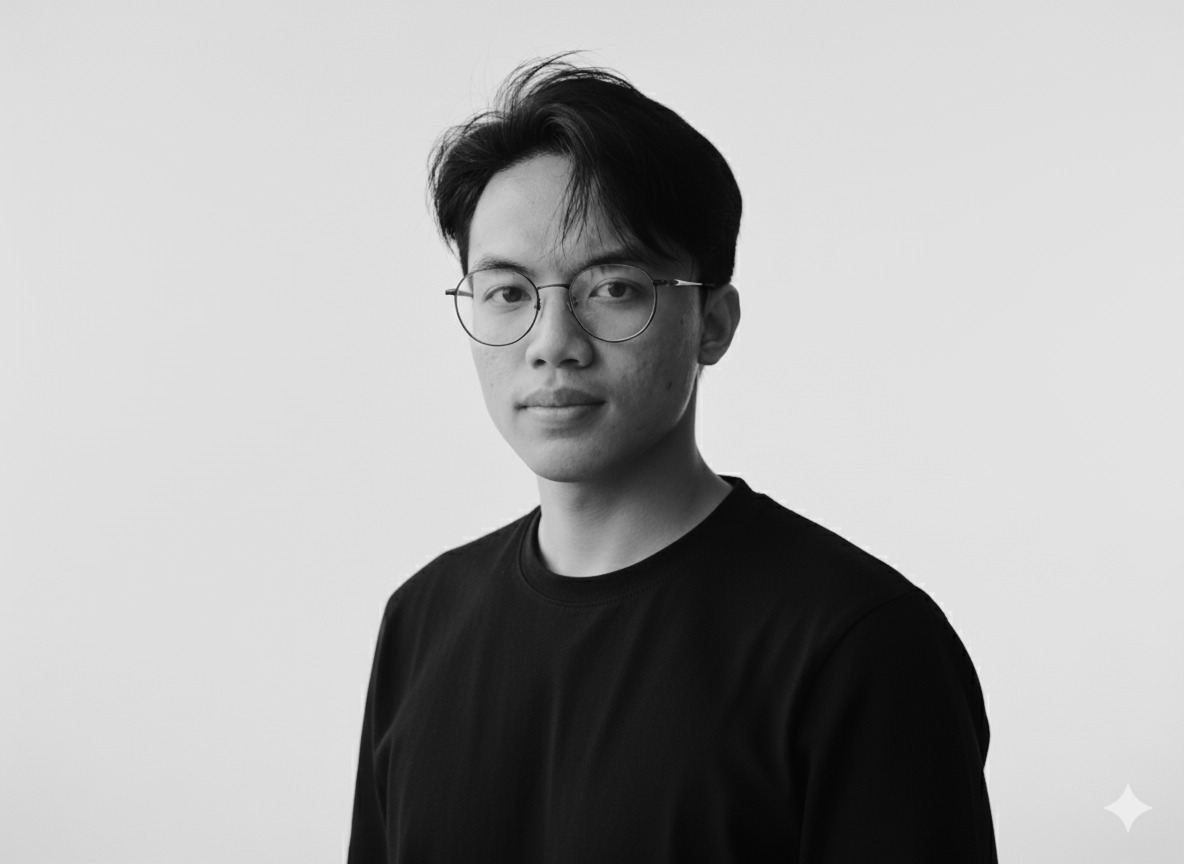
\includegraphics[width=1\linewidth,height=\textheight,keepaspectratio]{images/myself.jpg}

}

\caption{About me}

\end{figure}%

\begin{quote}
Jika ada sesuatu di ujung, maka saya akan mencarinya. Saya mencari
percikan semangat dan sebuah cahaya yang dapat membawa diri saya terus
ke arah dan jalan yang saya inginkan.
\end{quote}

Perkenalkan nama saya Muhammad Rizain Firdaus, sebuah anak yang selalu
ingin mencari kesempatan yang ideal bagi dirinya. Saya adalah anak
pertama yang lahir di keluarga yang sederhana, tidak kurang dan tidak
lebih. Umpamaan ini merupakan umpama yang saya rasa cukup adil untuk
mendeskripsikan hidup saya selama 20 tahun ini. Saya tumbuh sebagai anak
yang cukup unik dalam berpikir dan cenderung berbeda dengan pemikiran
orang-orang yang saya kenal. Uniknya saya memang mudah dalam beradaptasi
walaupun kadang membutuhkan waktu, hal ini saya refleksikan dari
perjalanan sekolah dan pertemanan saya yang saya alami selama lebih dari
12 tahun, 4 kali mengalami pindah sekolah, dan 8 sekolah berbeda dimulai
dari SD, SMP, SMA, dan sekarang kuliah.

\subsection*{Let's learn more about me}\label{lets-learn-more-about-me}
\addcontentsline{toc}{subsection}{Let's learn more about me}

\begin{itemize}
\tightlist
\item
  Untuk mengenal saya lebih lengkap, silakan kunjungi:

  \begin{itemize}
  \tightlist
  \item
    \textbf{\href{./All_About_me/index.qmd}{UTS-1: All About Me}}
  \end{itemize}
\item
  Untuk pandangan saya terhadap kehidupan melewati lagu:

  \begin{itemize}
  \tightlist
  \item
    \textbf{\href{./My_Stories_for_You/index.qmd}{UTS-3: My Stories for
    You}}
  \end{itemize}
\item
  Untuk mengenal analisis kepribadian saya:

  \begin{itemize}
  \tightlist
  \item
    \textbf{\href{./My_Shapes/index.qmd}{UTS-4: My SHAPE}}
  \end{itemize}
\end{itemize}

\bookmarksetup{startatroot}

\chapter{UTS-1 All About Me}\label{uts-1-all-about-me}

\section{Whats about me?}\label{whats-about-me}

Ketika saya menawarkan tentang diri saya, saya hanya berpikir mungkin
orang lain ingin mengenal diri saya dari sisi kepribadian seperti MBTI,
keunikan, maupun sebuah wawasan yang kita dapat bagi ke seluruh dunia
dan membuat diri kita merasa lebih baik. Oke, mungkin dari keunikan saya
terlebih dahulu lalu ke MBTI.

\subsection{My uniqueness}\label{my-uniqueness}

\begin{enumerate}
\def\labelenumi{\arabic{enumi}.}
\item
  \textbf{Saya handal dalam ``berimprovisasi'':} Maksud dari
  ``improvisasi'' di sini adalah kemampuan saya dalam ``meniru''
  seseorang. Tak jarang saya memiliki banyak panutan dalam hidup,
  dimulai dari orang yang saya looked up to hingga orang yang memang
  saya inginkan untuk menjadi seperti. Salah satu learning curve saya
  untuk menjadi pribadi yang lebih baik adalah belajar dari bagaimana
  seseorang yang sudah sukses di bidangnya dalam berperilaku, berbicara,
  dan berpikir. Sepanjang saya hidup saya merasa saya cenderung bersifat
  adaptif terhadap karakter saya. Maka dari ini saya kira, saya dapat
  fit in sesuai dengan lingkungan yang kadang 180 derajat berbeda dari
  lingkungan yang saya biasanya tinggali.
\item
  \textbf{Saya cenderung mendalami perasaan seseorang:} Mungkin ini
  termasuk sifat empatetik, namun diri saya kadang berpikir dan merasa
  dalam ketika saya ingin memahami seseorang. Dan ini tidak hanya
  terjadi di waktu tertentu saja, melainkan dari segala percakapan,
  interaksi, atau dampak dan sifat saya terhadap seseorang, saya
  cenderung memahami lebih terhadap seseorang dibandingkan memahami diri
  saya lebih lanjut. Mungkin borderlinenya adalah perilaku ini dekat
  dengan sifat judgemental atau perilaku menghakimi seseorang. Namun,
  tentunya tindakan tersebut tidak akan berdampak buruk lebih lanjut
  kecuali saya mengutarakan apa isi pikiran saya, saya merasa ada
  benefitnya juga dari sifat seperti ini yakni memiliki sifat empati
  mendalam dan cenderung menjaga perasaan seseorang.
\item
  \textbf{Saya lebih suka tepat sasaran:} Dahulu saya kira belajar 12-14
  jam akan berpengaruh pada sisi perspektif dan adaptabilitas otak saya,
  walaupun benar tetapi perspektif saya berubah semenjak kuliah. Waktu
  menentukan segalanya tetapi memanfaatkan waktu sebaik dan seefektif
  mungkin adalah jawabannya. Kepribadian saya adalah selalu melihat
  sesuatu untuk cepat selesai dan memiliki output yang tepat sasaran
  tidak berlebihan maupun tidak kurang. Walaupun banyak sekali yang
  harus saya pelajari di hidup ini, bagaimana mungkin saya pelajari
  semuanya? saya lebih merasa cocok apabila saya mempelajari jalan yang
  sesuai dengan diri saya.
\end{enumerate}

\subsection{MBTI}\label{mbti}

\begin{quote}
INFJ Saya memiliki pribadi yang introvert yakni cenderung lelah jika
terlalu banyak berinteraksi dengan orang lain dalam waktu sehari. Saya
memiliki intuisi dan juga terkadang lebih mengandalkan ke perasaan
dibandingkan berpikir logis. Dibalik itu kepribadian saya yang saya
jelaskan sebelumnya membuat saya memiliki kepribadian yang cukup
judgemental.
\end{quote}

\bookmarksetup{startatroot}

\chapter{UTS-2 My Songs for You}\label{uts-2-my-songs-for-you}

\section{Up and Downs}\label{up-and-downs}

\textbf{Fix You}\\
by \textbf{\emph{Coldplay}}

When you try your best, but you don't succeed\\
When you get what you want, but not what you need\\
When you feel so tired, but you can't sleep\\
Stuck in reverse

And the tears come streaming down your face\\
When you lose something you can't replace\\
When you love someone, but it goes to waste\\
Could it be worse?

Lights will guide you home And ignite your bones And I will try to fix
you

{[}\ldots{]}

And high up above or down below\\
When you're too in love to let it go\\
But if you never try, you'll never know\\
Just what you're worth

Lights will guide you home\\
And ignite your bones\\
And I will try to fix you

{[}\ldots{]}

Tears stream down your face\\
When you lose something you cannot replace\\
Tears stream down your face, and I

Tears stream down your face\\
I promise you I will learn from my mistakes\\
Tears stream down your face, and I

Lights will guide you home\\
And ignite your bones\\
And I will try to fix you

\section{Artistik}\label{artistik}

\textbf{Novacane} by \textbf{\emph{Frank Ocean}}

I think I started somethin'\\
I got what I wanted\\
Did-didn't, I can't feel nothin', superhuman\\
Even when I'm f*ckin', Viagra poppin'\\
Every single record, autotunin'\\
Zero emotion, muted emotion\\
Pitch-corrected, computed emotion, uh-huh

I blame it on the model broad with the Hollywood smile, aw\\
Stripper booty and a rack like wow\\
Brain like Berkeley, met her at Coachella\\
I went to see Jigga, she went to see Z Trip\\
.. Perfect

I took a seat on the ice-cold lawn\\
She handed me an ice blue bong, whatever\\
She said she wanna be a dentist really badly\\
She's in school paying for tuition doing p*rn in the Valley\\
At least you working, but girl, I can't feel my face\\
What are we smokin' anyway?\\
She said, ``Don't let the high go to waste''\\
But can you taste a little taste of

Novacane, baby, baby\\
Novacane, baby, I want you\\
f\emph{ck me good, f}ck me long, f*ck me numb\\
Love me now, when I'm gone love me none\\
Love me none, love me none\\
Numb, numb, numb, numb

Sink full of dishes, pacing in the kitchen\\
Cocaine for breakfast, yikes\\
Bed full of women\\
Flip on a tripod, little red light on\\
Shooting, I'm feeling like Stanley Kubrick\\
This is some visionary shit\\
Been tryna film pleasure with my eyes wide shut, but it keeps on moving

I blame it on the model broad with the Hollywood smile\\
Stripper booty with a rack like wow\\
I'll never forget you\\
You put me on a feeling I never had, never had, never had (never)\\
And ever since I've been tryna get it back\\
You pick it up and put it back\\
Now I'm something like the chemist on campus\\
But there's no drug around\\
Quite like what I found in you, you\\
I still can't feel my face (oh-oh)\\
What am I smokin' anyway? (Ah)\\
She said, ``Don't let the high go to waste'' (oh-oh)\\
But can you taste a little taste of?

Novacane, baby, baby (oh)\\
Novacane, baby, I want you\\
F\emph{ck me good, f}ck me long, f*ck me numb\\
Love me now, when I'm gone, love me none\\
Love me none, love me none\\
Numb, numb, numb, numb\\
Novacane, Novacane, Novacane, Novacane, Novacane (oh, oh, oh)\\
Numb the pain, numb the pain, numb the pain\\
Numb the pain, numb the pain (yeah)\\
Novacane, Novacane, Novacane, Novacane, Novacane (oh, ho)\\
For the pain, for the pain (ooh, huh)\\
Novacane, Novacane

Oh-huh, oh-huh, ho-huh\\
Oh-huh, oh-ho, ho-ho-huh\\
Oh-huh, oh-huh, ho-huh\\
Oh-huh, oh-ho, ho-ho-huh

Pretty girls involved with me\\
Makin' pretty love to me, pretty, pity, pity\\
All the pretty girls involved with me\\
Makin' pretty love to me, pretty, pity, pity\\
I can't feel a thing\\
I can't feel, can't feel a thing\\
Can't feel a thing, can't feel, feel, feel, feel her\\
I can't feel, feel her\\
Novacane, Novacane, Novacane\\
I can't feel, feel her\\
Novacane for the pain, for the pain\\
I can't, can't feel, feel her, feel her, oh\\
Novacane, Novacane, cane, cane, cane

\section{Takes on the song}\label{takes-on-the-song}

Lagu pertama \textbf{Fix You}, feelingnya mellow, haru, sedih, dan
harapan. Lagu ini merepresentasikan bagaimana dunia yang kadang kejam
membawakan banyaknya kesedihan dibandingkan kebahagiaan, namun dibalik
itu lagu ini merepresentasikan kepercayaan akan apa yang sudah dilalui
bukanlah hal yang sia-sia, melainkan sebuah langkah untuk memperbaiki
keadaan dan menjadi yang lebih baik. Lagu ini juga membuktikan bahwa
sesimpel dan sesederhana ritme, chord, struktur sebuah lagu dapat
memberikan dampak yang luar biasa terhadap psikologis seseorang. Sama
halnya dengan hidup yang cenderung bervariasi dan terdiri dari kejutan
akan ups and downs, tekanan yang dihadapi merupakan sebuah chorus dari
lagu ini yakni sebuah momen berulang yang selalu kita rasakan namun
tidak bisa dihindari. Namun dengan chorus ini, mereka memiliki tujuan
yakni tujuan sebagai sebuah jembatan menuju sebuah reff atau drop yang
akan membuat kita sadar bahwa inilah momennya, inilah saatnya, dan
sebuah kemenangan baik itu berupa harapan atau kejelasan akan jawaban,
inilah indahnya lagu ini.

Sedangkan, \textbf{Novacane} terdengar jauh berbeda dan memiliki tempo
yang lebih cepat. Lagu ini merepresentasikan bagaimana seseorang yang
memiliki daya atau kemampuan kreatif akan menguasai dunia. Apapun
bentuknya sesuatu yang sifatnya simpel seperti instrument dari lagu ini
yang hanya bersifat repetitif 1/1 dan bass yang cukup simpel membuktikan
bahwa dunia tidak butuh hal yang bersifat kompleks untuk membuktikan
sesuatu, melainkan daya kreatiflah yang akan menunjukkan jalan yang
tidak terduga. Sama layaknya lagu ini yang menjadi fokusnya adalah
lyricnya yang sangat terformat dengan baik dan rapih. Uniknya lagi, lagu
ini hanya menceritakan sebuah kejadian dari artis tersebut yang terjadi
di suatu hari dan suatu saat yang mungkin bisa dibilang hanya terjadi
1-2 jam saja, namun dikemas dengan lagu berdurasi 5 menit 2 detik dan
akan diingat selamanya.

\bookmarksetup{startatroot}

\chapter{UTS-3 My Stories for You}\label{uts-3-my-stories-for-you}

\begin{quote}
Stories are made to be remembered, not to be forgotten.
\end{quote}

\section{Proses Mencari Jati Diri}\label{proses-mencari-jati-diri}

\textbf{\emph{``Siapakah diri saya?''}}\\
Sebuah perjalanan dalam mengenal diri saya yang sebenarnya. Awal hidup
saya yang biasa-biasa saja, banyaknya kesalahan yang saya lakukan dan
alami berdampak pada perspektif terhadap diri saya yang sebenarnya.

Berawal ketika saya mengalami kesulitan dalam mengenali diri dan apa
yang saya inginkan untuk menjadi kedepannya. Namun, walaupun sampai
sekarang saya masih belum menemukan jawabannya. Hidup saya berputar pada
sebuah pertanyaan bukan jawaban. Semakin saya mencari tahu jawabannya,
semakin banyak pertanyaan yang saya miliki.

Akhir Desember tahun 2024 saya mulai untuk mencari hobi dan kesenangan
lainnya, saya memulai untuk mempelejari design dan UI/UX lalu
mendapatkan landing intern saya pertama di BAWASLU. Menjelang masa
magang saya merasa bahwa ketertarikan saya dengan teknologi semakin
kuat. Lalu sampai sekarang, saya masih mencari jawaban apa gunanya saya
lahir di dunia ini? apa tuuan dan manfaat saya yang saya bisa tinggalkan
di dunia ini selain ibadah? pertanyaan inilah yang akan terus saya
tanyakan.

\begin{quote}
Pesan yang diambil: ``Mencari jati diri sendiri sama seperti mencari
emas di gunung''
\end{quote}

\section{Bekas Luka Tanganku}\label{bekas-luka-tanganku}

\textbf{\emph{Fun fact: aku memiliki bekas luka sobek di tangan
kananku}}\\
Sejak saya berusia 2 tahun saya sudah memiliki bekas luka yang mendalam
di tangan kanan saya. Saya pun tidak ingat kejadiannya, namun saya
seringkali mendapatkan cerita dari mana bekas luka tangan tersebut
berasal.

Berawal ketika saya masih sangat lincah sebagai anak kecil. Yap, cukup
lincah, tidak bisa diam, tapi tidak nakal ;D.\\
Soal nakal\ldots{} mungkin tindakan saya yang ini bisa dibilang
sebaliknya. Saat itu, saya sedang berlari -larian, sesaat tepat di dapur
saya tidak sengaja menabrak bibi saya saat mencuci piring.\\
Tak disangka kejadiannya terjadi ketika bibi saya sedang memegang piring
di tangannya dan nasib buruknya piring tersebut merupakan piring kaca.
Piring itu pun jatuh dan menimpa tepat dekat urat nadi di tangan kanan
saya.

Semua orang rumah, saat itu panik dan langsung mengantarkan saya ke
rumah sakit. Tak ada opsi lain, saya pun harus dioperasi dan memastikan
pendarahan saya agar tidak menyebabkan saya kehilangan banyak darah. Dan
dari situlah terbit bekas luka yang sudah hampir 21 tahun saya miliki di
tangan kanan saya, kini kami berteman dan saya seringkali tidak lupa dan
mengkaitkan bekas luka tersebut sebagai memori berkesan waktu saya
kecil.

\begin{quote}
Pesan yang diambil: ``Tanggapilah kecelakaan sebagai sebuah cerita,
bukan penyesalan''
\end{quote}

\section{Selalu Erat dengan Musik}\label{selalu-erat-dengan-musik}

\textbf{\emph{Fun fact: saya memiliki 3 lagu yang fully di produced dan
telah dipublished}}\\
COVID-19 adalah penyebab saya menjadi suka dengan musik. Musik adalah
bahasa perasaan alam-semesta dan karya manusia yang paling saya kagumi.
Sejak SMA dan berkat COVID-19 saya menjadi tertarik dan mulai mendalami
composing dan producing. Hanya sebatas laptop kecil dan sebuah midi
piano di kamar kecil saya, saya tidak pernah berhenti untuk membuat
musik. Sampai sekarang pun saya masih memiliki niat dan keinginan untuk
membuat musik.

\begin{quote}
Pesan yang diambil: ``Carilah kesenangan dan kembali kepadanya''
\end{quote}

\bookmarksetup{startatroot}

\chapter{UTS-4 My SHAPE}\label{uts-4-my-shape}

Mengenai diri dari scope framework SHAPE (Spiritual Gifts, Heart,
Abilities, Personally, dan Experiences)

\section{My SHAPE (Spiritual Gifts, Heart, Abilities, Personality,
Experiences)}\label{my-shape-spiritual-gifts-heart-abilities-personality-experiences}

\subsection{S --- Spiritual Gifts
(Karunia)}\label{s-spiritual-gifts-karunia}

\begin{itemize}
\tightlist
\item
  Teaching \& Encouragement: suka menjelaskan dan menyalakan semangat
  orang lain.
\item
  Leadership in self-learning: membangun arah, disiplin, dan fokus pada
  ``tepat sasaran''.
\item
  Empathy \& Discernment: peka pada perasaan/cerita orang lain, mencoba
  memahami lebih dalam.
\item
  Creativity: improvisasi, bercerita, dan komposisi musik.
\end{itemize}

\subsection{H --- Heart (Minat \&
Kepedulian)}\label{h-heart-minat-kepedulian}

\begin{itemize}
\tightlist
\item
  Pengembangan diri yang bernilai: mencari ``cahaya''/arah dan
  kesempatan yang ideal.
\item
  Musik \& narasi: menggunakan lagu/cerita untuk menyalurkan emosi dan
  makna.
\item
  Desain \& teknologi: ketertarikan pada UI/UX dan teknologi yang
  membantu orang.
\item
  Relasi \& komunitas: menghargai koneksi yang hangat dan bermakna.
\end{itemize}

\subsection{A --- Abilities (Kemampuan)}\label{a-abilities-kemampuan}

\begin{itemize}
\tightlist
\item
  Adaptasi cepat: terbiasa pindah lingkungan/sekolah → mudah
  menyesuaikan diri.
\item
  Improvisasi \& modeling: ``meniru'' teladan baik untuk mempercepat
  belajar.
\item
  Komunikasi tulisan: merangkai narasi pribadi yang jujur dan reflektif.
\item
  Produksi kreatif: composing/producing musik; eksplorasi desain UI/UX.
\end{itemize}

\subsection{P --- Personality
(Kepribadian)}\label{p-personality-kepribadian}

\begin{itemize}
\tightlist
\item
  Vision-seeking \& purpose-driven: selalu mencari makna/arah jangka
  panjang.
\item
  Focused \& efficient: menyukai hasil tepat sasaran, tidak
  bertele-tele.
\item
  Introvert-reflektif: butuh ruang untuk memproses, namun empatik dan
  hangat.
\item
  Resilient: memaknai ``ups and downs'' sebagai bagian dari pertumbuhan.
\end{itemize}

\subsection{E --- Experiences
(Pengalaman)}\label{e-experiences-pengalaman}

\begin{itemize}
\tightlist
\item
  Lintas sekolah/lingkungan (8 sekolah): melatih adaptasi \& perspektif.
\item
  Proyek musik: merilis karya, belajar produksi dari perangkat
  sederhana.
\item
  Eksplorasi UI/UX \& magang: memantapkan minat pada teknologi dan
  desain.
\item
  Peristiwa pribadi (bekas luka, kisah hidup): membentuk ketangguhan dan
  empati.
\end{itemize}

\bookmarksetup{startatroot}

\chapter{UTS-5 My Personal Reviews}\label{uts-5-my-personal-reviews}

ChatGPT melakukan self-assessment UTS-1 s.d. UTS-5 langsung dari laman
yang Anda berikan dan menilai memakai rubrik tugas UTS (skala 1--5 per
kriteria). Rekap skor siap diunduh sebagai CSV:
\href{sandbox:/mnt/data/UTS_self_assessment.csv}{Download CSV
ringkasan}.

\bookmarksetup{startatroot}

\chapter{Hasil Self-Assessment UTS (URL:
ii-2100.github.io/all-about-me)}\label{hasil-self-assessment-uts-url-ii-2100.github.ioall-about-me}

Peer Assessment : {[}Google Sheets{]}
(https://docs.google.com/spreadsheets/d/1SVWRtD-\_EDtrOtqIhS2rm8KQwUINWwmq/edit?usp=sharing\&ouid=109573615308050881937\&rtpof=true\&sd=true)
\#\# Identifikasi

\begin{itemize}
\tightlist
\item
  \textbf{Nama \& NIM penulis:} Muhammad Rizain Firdaus - 13523164\\
\item
  \textbf{Penilai:} Self-Assessment menggunakan AI (Skor 2)\\
\item
  \textbf{Cakupan:} Portofolio berisi halaman UTS-1 (\emph{All About
  Me}), UTS-2 (\emph{My Songs for You}), UTS-3 (\emph{My Stories for
  You}), UTS-4 (\emph{My SHAPE}), dan UTS-5 (\emph{My Personal
  Reviews}).
\end{itemize}

\begin{center}\rule{0.5\linewidth}{0.5pt}\end{center}

\section{Tinjauan Umum}\label{tinjauan-umum}

Karya UTS menampilkan refleksi diri yang konsisten dan naratif.\\
UTS-1 menunjukkan kedalaman makna personal, UTS-2 menghubungkan musik
dengan nilai hidup, UTS-3 menggambarkan perjalanan keberanian dan
kegagalan, UTS-4 menyintesis potensi diri, sedangkan UTS-5 menilai
kembali proses tersebut secara kritis.

\begin{center}\rule{0.5\linewidth}{0.5pt}\end{center}

\section{Tinjauan Spesifik + Skor (1 --
5)}\label{tinjauan-spesifik-skor-1-5}

\subsection{\texorpdfstring{\textbf{UTS-1 --- All About
Me}}{UTS-1 --- All About Me}}\label{uts-1-all-about-me-1}

\begin{longtable}[]{@{}lll@{}}
\toprule\noalign{}
Kriteria & Deskripsi & Skor \\
\midrule\noalign{}
\endhead
\bottomrule\noalign{}
\endlastfoot
Orisinalitas & Narasi personal yang jujur dan unik. & 5 \\
Keterlibatan & Menarik dari awal hingga akhir. & 5 \\
Humor & Ringan dan relevan. & 3 \\
Wawasan & Memberi pemahaman mendalam tentang diri. & 5 \\
\textbf{Total} & & \textbf{18 / 20 (90 \%)} \\
\end{longtable}

\subsection{\texorpdfstring{\textbf{UTS-2 --- My Songs for
You}}{UTS-2 --- My Songs for You}}\label{uts-2-my-songs-for-you-1}

\begin{longtable}[]{@{}lll@{}}
\toprule\noalign{}
Kriteria & Deskripsi & Skor \\
\midrule\noalign{}
\endhead
\bottomrule\noalign{}
\endlastfoot
Orisinalitas & Mengaitkan lagu dengan pengalaman pribadi. & 4 \\
Keterlibatan & Emosional dan menyentuh. & 5 \\
Humor & Ringan, tidak dominan. & 3 \\
Inspirasi & Menginspirasi rasa syukur dan kenangan. & 4 \\
\textbf{Total} & & \textbf{16 / 20 (80 \%)} \\
\end{longtable}

\subsection{\texorpdfstring{\textbf{UTS-3 --- My Stories for
You}}{UTS-3 --- My Stories for You}}\label{uts-3-my-stories-for-you-1}

\begin{longtable}[]{@{}lll@{}}
\toprule\noalign{}
Kriteria & Deskripsi & Skor \\
\midrule\noalign{}
\endhead
\bottomrule\noalign{}
\endlastfoot
Orisinalitas & Cerita jujur dan segar. & 5 \\
Keterlibatan & Alur emosional dan hidup. & 5 \\
Pengembangan Narasi & Tiap bagian tersambung baik. & 4 \\
Inspirasi & Pesan kuat tentang keberanian dan pertumbuhan. & 5 \\
\textbf{Total} & & \textbf{19 / 20 (95 \%)} \\
\end{longtable}

\subsection{\texorpdfstring{\textbf{UTS-4 --- My
SHAPE}}{UTS-4 --- My SHAPE}}\label{uts-4-my-shape-1}

\begin{longtable}[]{@{}lll@{}}
\toprule\noalign{}
Kriteria & Deskripsi & Skor \\
\midrule\noalign{}
\endhead
\bottomrule\noalign{}
\endlastfoot
Orisinalitas & Sintesis unik nilai \& visi diri. & 5 \\
Keterlibatan & Naratif menarik dan reflektif. & 5 \\
Pengembangan Narasi & Struktur SHAPE logis \& terpadu. & 5 \\
Inspirasi & Mendorong pembaca mengenal diri. & 5 \\
\textbf{Total} & & \textbf{20 / 20 (100 \%)} \\
\end{longtable}

\begin{center}\rule{0.5\linewidth}{0.5pt}\end{center}

\section{\texorpdfstring{\textbf{Rekap Skor
Ringkas}}{Rekap Skor Ringkas}}\label{rekap-skor-ringkas}

\begin{longtable}[]{@{}
  >{\raggedright\arraybackslash}p{(\linewidth - 4\tabcolsep) * \real{0.2222}}
  >{\raggedright\arraybackslash}p{(\linewidth - 4\tabcolsep) * \real{0.2963}}
  >{\raggedright\arraybackslash}p{(\linewidth - 4\tabcolsep) * \real{0.4815}}@{}}
\toprule\noalign{}
\begin{minipage}[b]{\linewidth}\raggedright
UTS
\end{minipage} & \begin{minipage}[b]{\linewidth}\raggedright
Total
\end{minipage} & \begin{minipage}[b]{\linewidth}\raggedright
Persentase
\end{minipage} \\
\midrule\noalign{}
\endhead
\bottomrule\noalign{}
\endlastfoot
UTS-1 & 18 / 20 & 90 \% \\
UTS-2 & 16 / 20 & 80 \% \\
UTS-3 & 19 / 20 & 95 \% \\
UTS-4 & 20 / 20 & 100 \% \\
\textbf{Total Rata-rata } & & \textbf{≈ 91,25 \% (baik sekali untuk UTS
1-4)} \\
\end{longtable}

\begin{center}\rule{0.5\linewidth}{0.5pt}\end{center}

\bookmarksetup{startatroot}

\chapter{UAS-1 My Concepts}\label{uas-1-my-concepts}

Mau hidup epik ? \href{lifestory.pdf}{Write your Life Story}

Apa itu berkonsep?

\url{https://youtu.be/QVfUlVBO80U?si=yM6q_rwV9rcDBbu7}

\bookmarksetup{startatroot}

\chapter{UAS-3 My Opinions}\label{uas-3-my-opinions}

SApa itu beropini? \href{BM\%20Opini.mp4}{Opini Berpengaruh}

Bagiamana menjaadi menarik? \href{./Interesting.mp4}{Menjadi Menarik}

\bookmarksetup{startatroot}

\chapter{UAS-3 My Innovations}\label{uas-3-my-innovations}

\bookmarksetup{startatroot}

\chapter{UAS-4 My Knowledge}\label{uas-4-my-knowledge}

Cara saya mengkomunikasikan sebuah pengatahuan sebagai petunjuk bagi
orang lain 1) saya tulis
\href{Rekomendasi\%20Presentasi\%20Efektif(Contoh\%20Makalah).pdf}{makalah
sebagai bahan utama} 2) lalu saya buat
\href{Contoh\%20Transkrip\%20Presentasi.pdf}{transkrip ucapan lisan} 3)
kemudian saya kembangkan
\href{Rekomendasi\%20Presentasi\%20(Contoh\%20Slides).pdf}{slide
pendukung trnsskrip} 4) lalu saya memproduksivideo audio visual
\url{https://youtu.be/ZbghfMvnPZc} \url{https://youtu.be/ZbghfMvnPZc}

\bookmarksetup{startatroot}

\chapter{UTS-5 My Personal Reviews}\label{uts-5-my-personal-reviews-1}

Berikut cara saya melakukan review: mengguan chatGPT, saya mengattach
\href{skor_uts.pdf}{file promt ChatGPT}, disertai perintah :``self
assess uts-1 sanpai uts-5 dari URL
`https://ii-2100.github.io/all-about-me/'\,''

ChatGPT melakukan self-assessment UTS-1 s.d. UTS-5 langsung dari laman
yang Anda berikan dan menilai memakai rubrik tugas UTS (skala 1--5 per
kriteria). Rekap skor siap diunduh sebagai CSV:
\href{sandbox:/mnt/data/UTS_self_assessment.csv}{Download CSV
ringkasan}.

\bookmarksetup{startatroot}

\chapter{Hasil Self-Assessment UTS (URL:
ii-2100.github.io/all-about-me)}\label{hasil-self-assessment-uts-url-ii-2100.github.ioall-about-me-1}

\section{Identifikasi}\label{identifikasi}

\begin{itemize}
\tightlist
\item
  Nama \& NIM penulis: \textbf{Muhammad Rizain Firdaus - 13523164}
\item
  Penilai: \textbf{Self-assessment (ChatGPT)}
\end{itemize}

\section{Tinjauan Spesifik + Skor
(1--5)}\label{tinjauan-spesifik-skor-15}

\subsection{UTS-1 --- All About Me (di
beranda)}\label{uts-1-all-about-me-di-beranda}

\textbf{Skor per kriteria:} Orisinalitas \textbf{3}, Keterlibatan
\textbf{3}, Humor \textbf{1}, Wawasan/Insight \textbf{3} → \textbf{Total
10/20 (50\%)}. \textbf{Alasan singkat:} Perkenalan diri faktual dan
jelas, namun gaya masih informatif ketimbang naratif (minim humor dan
moment ``hook''). (\href{https://ii-2100.github.io/all-about-me/}{II
2100}) \textbf{Saran perbaikan:} Buka dengan anekdot pribadi (1--2
paragraf) yang ``mengikat'' (mis. titik balik karier/keluarga),
tambahkan satu momen humor ringan, lalu tutup dengan refleksi singkat
tentang nilai/visi diri agar aspek insight naik.

\subsection{UTS-2 --- My Songs for You}\label{uts-2-my-songs-for-you-2}

\textbf{Skor per kriteria:} Orisinalitas \textbf{2}, Keterlibatan
\textbf{2}, Humor \textbf{1}, Inspirasi \textbf{2} → \textbf{Total 7/20
(35\%)}. \textbf{Alasan singkat:} Halaman menampilkan judul lagu ``River
in my Mind'', ``Heaven on Earth'', namun tanpa lirik/cerita di balik
lagu sehingga sulit menilai aspek pesan, humor, dan inspirasi.
(\href{https://ii-2100.github.io/all-about-me/My_Song_for_You/index.html}{II
2100}) \textbf{Saran perbaikan:} Tambahkan lirik lengkap, 1 paragraf
cerita proses kreatif, dan 2--3 kalimat ``pesan untukmu'' agar inspirasi
terbaca; sertakan player/tautan yang dapat diputar langsung + fallback
transkrip.

\subsection{UTS-3 --- My Stories for
You}\label{uts-3-my-stories-for-you-2}

\textbf{Skor per kriteria:} Orisinalitas \textbf{5}, Keterlibatan
\textbf{5}, Pengembangan Narasi \textbf{4}, Inspirasi \textbf{5} →
\textbf{Total 19/20 (95\%)}. \textbf{Alasan singkat:} Cerita ``Gaun
Pengantin Gladys'' dkk sangat personal, emosional, dan inspiratif; ritme
bertutur hidup serta detail situasional kuat (konten ramu unsur
penebusan/keluarga/iman).
(\href{https://ii-2100.github.io/all-about-me/My_Stories_for_You/index.html}{II
2100}) \textbf{Saran perbaikan:} Tambah ``lead'' 2--3 kalimat yang
merangkum pesan kunci tiap cerita; akhiri dengan ajakan/refleksi 1--2
kalimat agar resonansi ke pembaca makin jelas.

\subsection{UTS-4 --- My SHAPE}\label{uts-4-my-shape-2}

\textbf{Skor per kriteria:} Orisinalitas \textbf{1}, Keterlibatan
\textbf{1}, Pengembangan \textbf{1}, Inspirasi \textbf{1} →
\textbf{Total 4/20 (20\%)}. \textbf{Alasan singkat:} Konten belum
tersedia.
(\href{https://ii-2100.github.io/all-about-me/My_Shapes/index.html}{II
2100}) \textbf{Saran perbaikan (prioritas):}

\begin{enumerate}
\def\labelenumi{\arabic{enumi}.}
\tightlist
\item
  Tampilkan rekap SHAPE (Spiritual gifts, Heart, Abilities, Personality,
  Experiences) dalam 1 tabel ringkas + 3--5 butir bukti;
\item
  Narasikan 2 pengalaman kunci (±150 kata/each) yang menunjukkan
  ``signature strengths'';
\item
  Tutup dengan 3 rencana aksi konkret (who/what/when).
\end{enumerate}

\subsection{UTS-5 --- My Personal
Reviews}\label{uts-5-my-personal-reviews-2}

\textbf{Skor per kriteria:} Pemahaman Konsep \textbf{2}, Analisis Kritis
\textbf{1}, Argumentasi (Logos) \textbf{1}, Etos \& Empati \textbf{2},
Rekomendasi \textbf{1} → \textbf{Total 7/25 (28\%)}. \textbf{Alasan
singkat:} Halaman berisi metode cara menilai, tetapi \textbf{belum ada}
contoh \textbf{review personal} yang lengkap terhadap sebuah pesan/teks
sehingga aspek analisis-argumentasi tak terbaca.
(\href{https://ii-2100.github.io/all-about-me/My_Personal_Reviews/index.html}{II
2100}) \textbf{Saran perbaikan:} Pilih 1 karya personal (mis.
UTS-1/2/3), tulis review 400--600 kata: ringkas pesan, nilai dengan
rubrik, berikan 2--3 bukti kutipan, evaluasi etos/empati, lalu tutup
dengan rekomendasi perbaikan spesifik.

\begin{center}\rule{0.5\linewidth}{0.5pt}\end{center}

\section{Rekap Skor (ringkas)}\label{rekap-skor-ringkas-1}

\begin{itemize}
\tightlist
\item
  \textbf{UTS-1:} 10/20 → \textbf{50\%}
\item
  \textbf{UTS-2:} 7/20 → \textbf{35\%}
\item
  \textbf{UTS-3:} 19/20 → \textbf{95\%}
\item
  \textbf{UTS-4:} 4/20 → \textbf{20\%}
\item
  \textbf{UTS-5:} 7/25 → \textbf{28\%}
\end{itemize}

CSV lengkap sudah saya siapkan untuk dokumentasi dan olah lanjut:
\href{sandbox:/mnt/data/UTS_self_assessment.csv}{Download CSV
ringkasan}.

\section{Langkah Perbaikan Cepat (prioritas 1
minggu)}\label{langkah-perbaikan-cepat-prioritas-1-minggu}

\begin{enumerate}
\def\labelenumi{\arabic{enumi}.}
\tightlist
\item
  \textbf{Lengkapi UTS-4 (My SHAPE)} sesuai saran di atas;
\item
  \textbf{Tambahkan lirik + sinopsis} untuk tiap lagu di UTS-2 agar bisa
  dinilai isi/inspirasinya;
\item
  \textbf{Tulis 1 review personal penuh} (UTS-5) memakai rubrik (pilih
  salah satu karya Anda sendiri sebagai objek);
\item
  Revisi UTS-1 dengan pembuka anekdot + refleksi nilai diri.
\end{enumerate}

Jika Anda mau, saya bisa bantu merapikan UTS-4 (tabel SHAPE + narasi)
dan membuat kerangka cepat untuk \textbf{review} di UTS-5 dari salah
satu karya Anda.

\bookmarksetup{startatroot}

\chapter{Summary}\label{summary}

In summary, this book has no content whatsoever.

\bookmarksetup{startatroot}

\chapter*{References}\label{references}
\addcontentsline{toc}{chapter}{References}

\markboth{References}{References}

\phantomsection\label{refs}




\end{document}
